\section{Evaluation}

In this section, we introduce our experiment of \TheName{} and evaluate the effectiveness and overhead of our system. 

\subsection{Experiment Setup}
We use hardware SDN switch to test our approach. Floodlight, OpenFlow controller running our application, are deployed in an Intel Xeon Quad-Core CPU E5504 and 4GB RAM machine. We deploy two commercial hardware OpenFlow switch, EdgeCore AS4610-54T, in our hardware testbed, and the maximum transmitting rate of each port in the switch $R_m$ is 1 Gbps. We implement the attack in C code to generate the low-rate TCP attack with different $T$ and $L$. 

Figure~\ref{fig:topology} shows the topology of our testbed. $h_1$ generates the legitimate traffic as background traffic and $h_3$ receives the traffic. $h_2$ is generate the low-rate TCP attack traffic to $h_4$. The bandwidth of the link between $S_1$ and $S_2$ is overloaded and the queue of $S_1$ are congested for the period burst packet. The TCP flows affected seriously by low-rate TCP attack.

\begin{figure}
\vspace{-0.1in}
\centering
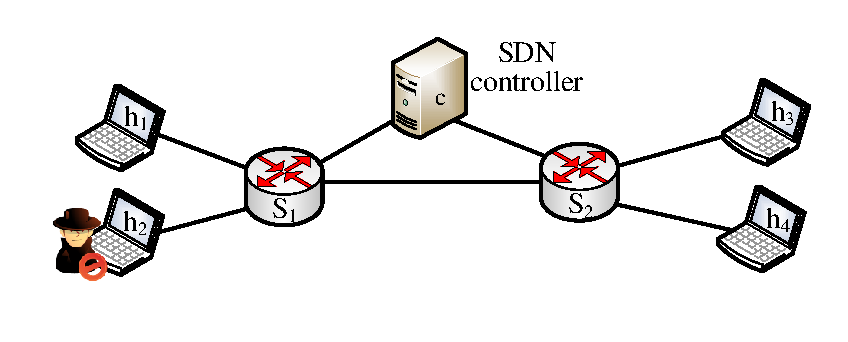
\includegraphics[width=3.4in]{Evaluation/topology.pdf}
\vspace{-0.1in}
\caption{\small{The network topology of our testbed.}}
\label{fig:topology}
\vspace{-0.2in}
\end{figure}

\subsection{Accuracy and Robustness}

We first measure the period by analyzing the statistics obtained from the counters associated with the active ports. After obtaining the sequence of the rate, we use the thresholding method to obtain the binary signals and measure the period of the signals. If there exists the low-rate TCP attack in a port, the measured period will be a positive value. Otherwise, the measured period will be zero. We compare the measured period of signals with the period of the low-rate TCP attack and obtain the error of the measurement.

\begin{figure}
\vspace{0in}


\begin{minipage}[t]{0.49\linewidth}
\centering
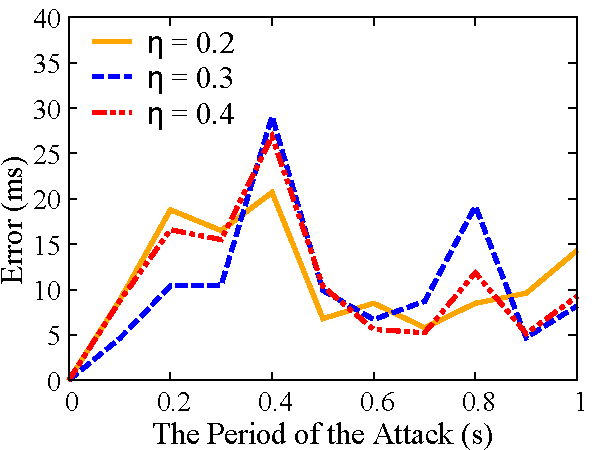
\includegraphics[width=1.7in]{Evaluation/period.pdf}
\caption{\small{Measurement error}}
\label{fig:period}
\end{minipage}
\begin{minipage}[t]{0.49\linewidth}
\centering
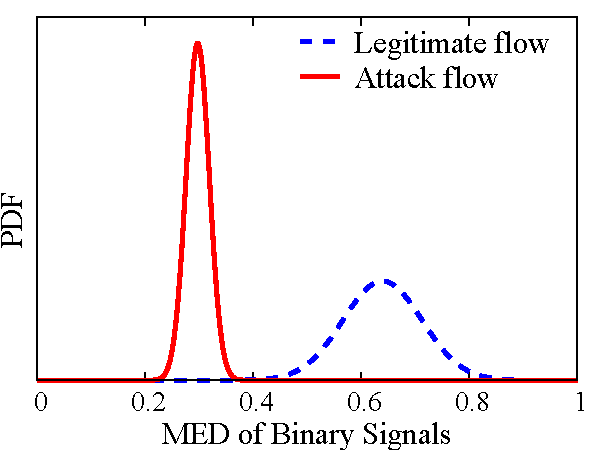
\includegraphics[width=1.7in]{Evaluation/distribution.pdf}
\caption{\small{PDF of MED}}
\label{fig:PDF}
\end{minipage}
\vspace{-0.2in}
\end{figure}

Figure~\ref{fig:period} shows the error of period measurement for various period values. We use Algorithm~\ref{alg:port_locate} to measure the period of the low-rate TCP attack. For the characteristics of the low-rate TCP attack, we consider $R $ = 1.1 Gbps. For the algorithm, we suppose that $T_{min}$  = 0.005s, $T_{max}$ = 0.64s, $\epsilon$ = 0.01. We set the period of the low-rate TCP attack from 0.1s to 1s. The periodicity of the flows can be detected and the period of the low-rate TCP attack is measured with the error ranging from 4 ms to 30 ms. Moreover, if none of the low-rate TCP attacks exist, the measured period and the error of the measurement will be zero. Furthermore, $T_s$ used for period measurement is also used for locating the attack hosts if the low-rate TCP attack exist.


For the appropriate threshold $\gamma$ to differentiate the legitimate and attack flows, the probability density function (PDF) of the MED between binary signals of potential flows and that of the affected ports is essential. Figure~\ref{fig:PDF} shows the PDF of MED for legitimate and attack traffic. The appropriate sampling period $T_s$ is obtained by the previous steps. We carry out an experiment to evaluate the MED between the binary signals of flow rule and that of the port. 
We consider the length of binary signals $N$=100, the period of the low-rate TCP attack $T$ is randomly chosen from [0.8,1.5], the burst length of the low-rate TCP attack $L$ is randomly chosen from (0, 0.4], and the burst rate is 1.1 Gbps. We generate 100 flows as legitimate flows. The MED of the attack flows basically ranges from 0.2 to 0.4 and the MED of the legitimate flows basically ranges from 0.4 to 0.9. In most cases, the MED of the attack flows is smaller than that of legitimate flows, because the majority of packets transmitted by the ports are the low-rate TCP attack packets. From Figure~\ref{fig:PDF}, A clear determination point (i.e. $MED$ = 0.4) can be obtained to differentiate attack flows from the legitimate flows.


Figure~\ref{fig:Performance} illustrates the performance of the binary classifier. We differentiate the attack flows by analyzing the similarity between the binary signals of the potential flows and that of ports. Considering the threshold $\gamma$ = 0.4. We sample the coming rate of ports for 5 $T_b$ measured before, classify them for the binary signals. We obtain MED between potential flows and the affected port by equation~(\ref{eq:euclidean_distance}) and differentiate the attack flows by $\gamma$. If the MED of a flow less than $\gamma$, we denote the flow as an attack flow. Otherwise, we denote the flow as a legitimate flow. We observe that attack flows detection have a recall rate of more than 90 percent and a false positive rate of less than 5 percent. Most of the attack flows are identified and the legitimate flows are not misidentified.


\begin{figure}
\vspace{0in}
\centering

\subfloat[\small{Recall rate}]{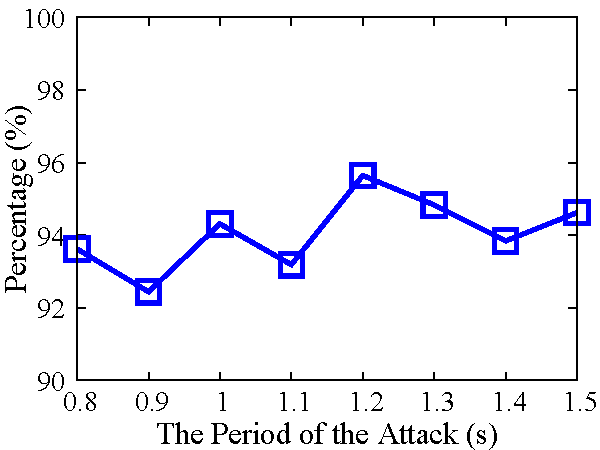
\includegraphics[width=1.7in]{Evaluation/recall.pdf}\label{fig:recall}}
\subfloat[\small{False positive rate}]{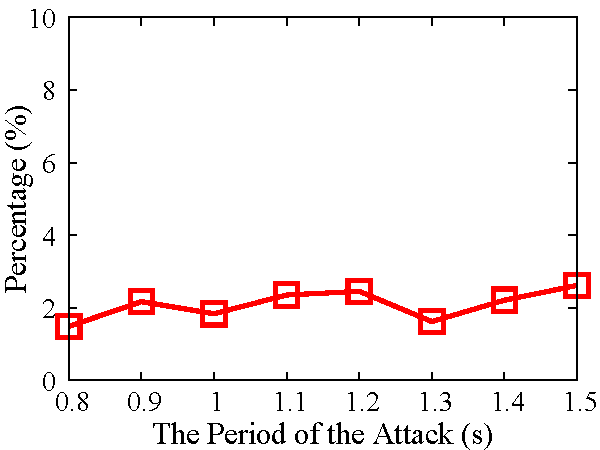
\includegraphics[width=1.7in]{Evaluation/false_positive.pdf}\label{fig:false_positive}}
\vspace{-0.1in}
\caption{\small{Performance.}}
\label{fig:Performance}
\vspace{-0.2in}
\end{figure}

\subsection{Evaluation of Defense Mechanism.} 
In this section, we show our evaluation on the effectiveness and overhead of \TheName{}. we first measure the throughput of a TCP flow with and without defense in the host. And then, we do the experiment for the CPU utilization with the low-rate TCP attacks with different periods.

\noindent \textbf{Effectiveness.}  We generate 100 TCP flows and they are transmitted by a port. we also generate the low-rate TCP attack traffic ($T$ = 210ms, $L$ = 90ms, $R$ = 1.1 Gbps) transmitted by the port. Figure~\ref{fig:throughput} shows a TCP flow throughput with and without attack. We record the throughput of a TCP flow on the host for 30 seconds. Under the low-rate TCP attack, the throughput of the TCP flow is almost zero. The reason is that the low-rate TCP attack forces the TCP flow to cause retransmission continuously. With the defense of \TheName{}, the low-rate TCP attack is mitigated at access switch. Hence, the TCP flow has a throughput of 8 Mbps.

\noindent \textbf{Overhead.} To evaluate the overhead of our system, we report the CPU utilization of the controller. We launch the low-rate TCP attack with $T$ from 0.1s to 1s and the flooding DoS. Figure~\ref{fig:utilizaition} shows that the overhead of \TheName{} with various period values. The controller overhead is increased because of the decrease of the period. According to the Nyquist theorem, the upper bound of the sampling period for the low-rate TCP attack is $T/2$, which means $T_s$ needs to be low enough for the low period values. Thus, the low period of the low-rate TCP attack incurs high overhead for the controller. If the attack is the flooding attack, the detection will terminate with a sampling period of $T_{min}$. \TheName{} introduces an additional CPU utilization of 25 percent at most. Such overhead is acceptable for deploying our defense system.

\begin{figure}
\begin{minipage}[t]{0.49\linewidth}
\centering
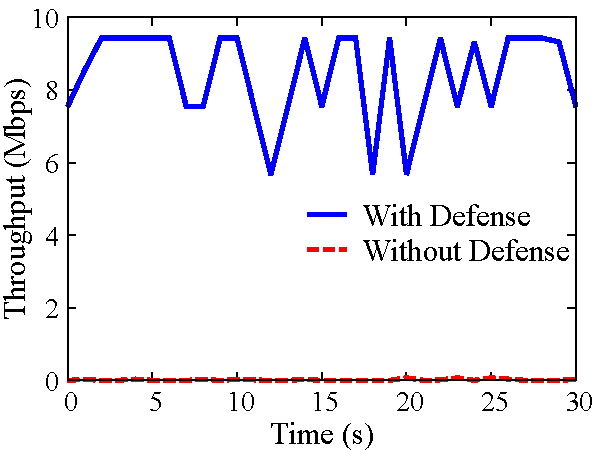
\includegraphics[width=1.7in]{Evaluation/throughput.pdf}
\caption{\small{The throughput with and without defense }}
\label{fig:throughput}
\end{minipage}
\begin{minipage}[t]{0.49\linewidth}
\centering
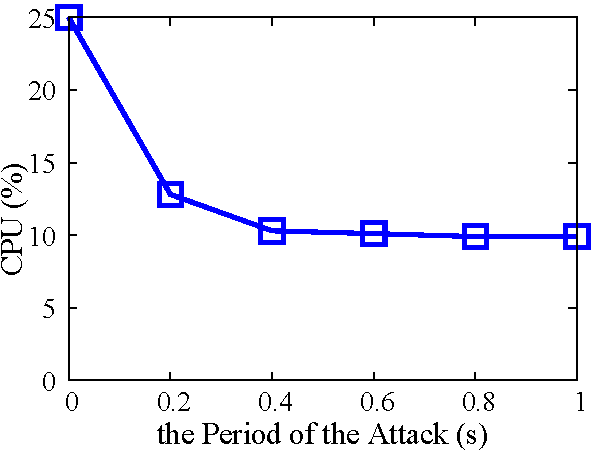
\includegraphics[width=1.7in]{Evaluation/utilizaition.pdf}
\caption{\small{CPU utilization}}
\label{fig:utilizaition}
\end{minipage}
\vspace{-0.2in}
\end{figure}


